\documentclass[tikz,border=5pt]{standalone}
\usepackage[dvipsnames]{xcolor}
\usepackage{tikz}
\usetikzlibrary{arrows.meta,calc,positioning,quotes,fit}

\tikzset{
  sccnode/.style={
    rectangle, rounded corners=3pt,
    draw=blue!50!black,
    minimum width=15mm, minimum height=10mm,
    font=\bfseries, inner sep=1pt
  },
  gen0fill/.style={fill=blue!12},
  gen1fill/.style={fill=orange!15},
  gen2fill/.style={fill=green!15},
  genlabel/.style={font=\small\itshape\bfseries, text=black!80, inner sep=1pt},
  connection/.style={thick, ->, >=Latex},
  metadata/.style={
    font=\ttfamily\small, align=left,
    draw=black!40, fill=white, rounded corners=2pt, inner sep=3pt
  },
  statelabel/.style={font=\small\bfseries, rotate=90},
  divider/.style={dashed, black!55},
  reloc/.style={
    ->, very thick, dashed, draw=red!70!black, >=Latex
  },
  reloclabel/.style={
    font=\small\ttfamily, text=red!70!black,
    fill=white, inner sep=2pt
  }
}

\begin{document}
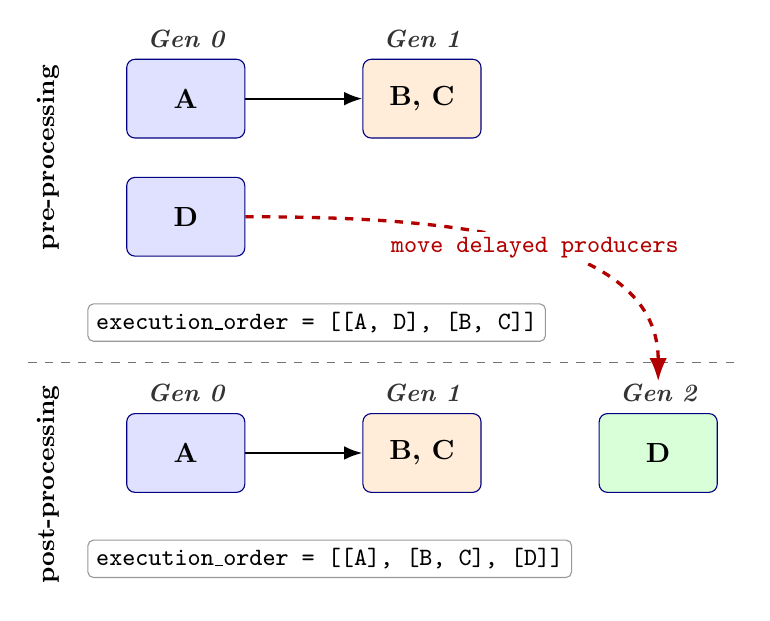
\begin{tikzpicture}
  %\draw[help lines, step=0.5] (-1.5,-1) grid (8.5,7);

  % ==== PRE-STATE (top) ====
  \node[statelabel] at (-0.5, 4.75) {pre-processing};
  \node[sccnode, gen0fill] (sA1)  at (1.25, 5.5) {A};
  \node[sccnode, gen0fill] (sD1)  at (1.25, 4)   {D};
  \node[sccnode, gen1fill] (sBC1) at (4.25, 5.5) {B, C};
  \draw[connection] (sA1) -- (sBC1);
  \node[genlabel, above=1mm of sA1.north]  {Gen 0};
  \node[genlabel, above=1mm of sBC1.north] {Gen 1};
  \node[metadata, anchor=north west] at (0, 2.9)
    {execution\_order = [[A, D], [B, C]]};

  % ==== DIVIDER ====
  \draw[divider] (-.75, 2.15) -- (8.3, 2.15);

  % ==== POST-STATE (bottom) ====
  \node[statelabel] at (-0.5, 0.6) {post-processing};
  \node[sccnode, gen0fill] (sA2)  at (1.25, 1) {A};
  \node[sccnode, gen1fill] (sBC2) at (4.25, 1) {B, C};
  \node[sccnode, gen2fill] (sD2)  at (7.25, 1) {D};
  \draw[connection] (sA2) -- (sBC2);
  \node[genlabel, above=1mm of sA2.north]  {Gen 0};
  \node[genlabel, above=1mm of sBC2.north] {Gen 1};
  \node[genlabel, above=1mm of sD2.north] (gen2)  {Gen 2};
  \node[metadata, anchor=north west] at (0, -0.1)
    {execution\_order = [[A], [B, C], [D]]};

  % ==== Single relocation arrow: shows movement AND names the operation ====
  \draw[reloc] (sD1.east)
    to[out=0, in=90, looseness=0.9]
    node[pos=0.55, reloclabel]
      {move delayed producers}
    (gen2.north);
\end{tikzpicture}
\end{document}
